\documentclass{beamer}
\usepackage[utf8]{inputenc}

\usetheme{Madrid}
\usecolortheme{default}
\usepackage{amsmath,amssymb,amsfonts,amsthm}
\usepackage{txfonts}
\usepackage{tkz-euclide}
\usepackage{listings}
\usepackage{adjustbox}
\usepackage{array}
\usepackage{tabularx}
\usepackage{gvv}
\usepackage{lmodern}
\usepackage{circuitikz}
\usepackage{tikz}
\usepackage{graphicx}

\setbeamertemplate{page number in head/foot}[totalframenumber]

\usepackage{tcolorbox}
\tcbuselibrary{minted,breakable,xparse,skins}



\definecolor{bg}{gray}{0.95}
\DeclareTCBListing{mintedbox}{O{}m!O{}}{%
	breakable=true,
	listing engine=minted,
	listing only,
	minted language=#2,
	minted style=default,
	minted options={%
		linenos,
		gobble=0,
		breaklines=true,
		breakafter=,,
		fontsize=\small,
		numbersep=8pt,
		#1},
	boxsep=0pt,
	left skip=0pt,
	right skip=0pt,
	left=25pt,
	right=0pt,
	top=3pt,
	bottom=3pt,
	arc=5pt,
	leftrule=0pt,
	rightrule=0pt,
	bottomrule=2pt,
	toprule=2pt,
	colback=bg,
	colframe=orange!70,
	enhanced,
	overlay={%
		\begin{tcbclipinterior}
			\fill[orange!20!white] (frame.south west) rectangle ([xshift=20pt]frame.north west);
	\end{tcbclipinterior}},
	#3,
}
\lstset{
	language=C,
	basicstyle=\ttfamily\small,
	keywordstyle=\color{blue},
	stringstyle=\color{orange},
	commentstyle=\color{green!60!black},
	numbers=left,
	numberstyle=\tiny\color{gray},
	breaklines=true,
	showstringspaces=false,
}
%------------------------------------------------------------
%This block of code defines the information to appear in the
%Title page
\title %optional
{1.9.25}
\date{}
%\subtitle{A short story}

\author % (optional)
{M Chanakya Srinivas- EE25BTECH11036}




\begin{document}


\frame{\titlepage}

%------------------- Frame 1 -------------------%


%---------------------------------------------------
\begin{frame}{Question}
\textbf{Question 1.9.25:}  
If the point $P(x,y)$ is equidistant from $A(a+b, b-a)$ and $B(a-b, a+b)$,  
prove that
\begin{align*}
    bx = ay
\end{align*}
\end{frame}

%---------------------------------------------------
\begin{frame}{Given Data}
Define
\begin{align}
\vec{z} &= \myvec{a \\ b}. 
\end{align}

Then
\begin{align}
\vec{A} &= \myvec{1 & 1 \\ -1 & 1}\vec{z}, \\
\vec{B} &= \myvec{1 & -1 \\ 1 & 1}\vec{z}, \\
\vec{P} &= \myvec{x \\ y}.
\end{align}

Notice that
\begin{align}
\myvec{1 & -1 \\ 1 & 1} 
= \myvec{1 & 1 \\ -1 & 1}^T 
\quad \Rightarrow \quad \vec{B} = \vec{A}^T \vec{z}.
\end{align}
\end{frame}

%---------------------------------------------------
\begin{frame}{Equidistant Condition}
\begin{align}
\norm{\vec{P}-\vec{A}}^2 &= \norm{\vec{P}-\vec{B}}^2 \\
(\vec{P}-\vec{A})^T(\vec{P}-\vec{A}) &= (\vec{P}-\vec{A}^T)^T(\vec{P}-\vec{A}^T)
\end{align}
\end{frame}

%---------------------------------------------------
\begin{frame}{Simplification}
Using $B=A^T$,
\begin{align}
2(\vec{A}^T - \vec{A})^T \vec{P} &= \vec{A}^{T}\vec{A}^{T} - \vec{A}^T\vec{A}.
\end{align}

But since $\vec{A}^T\vec{A}$ is symmetric,  
\begin{align}
\vec{A}^{T}\vec{A}^{T} - \vec{A}^T\vec{A} = 0.
\end{align}

Hence
\begin{align}
(\vec{A}^T - \vec{A})^T \vec{P} = 0.
\end{align}
\end{frame}

%---------------------------------------------------
\begin{frame}{Final Result}
Expanding,
\begin{align}
(\vec{B}-\vec{A})^T\vec{P} 
&= \Bigg(\myvec{0 & -2 \\ 2 & 0}\vec{z}\Bigg)^T \vec{P}, \\
&= -2bx + 2ay = 0, \\
\Rightarrow \quad bx &= ay
\end{align}
\end{frame}
















\begin{frame}{Plot by shared output}
    

\begin{figure}
    \centering
    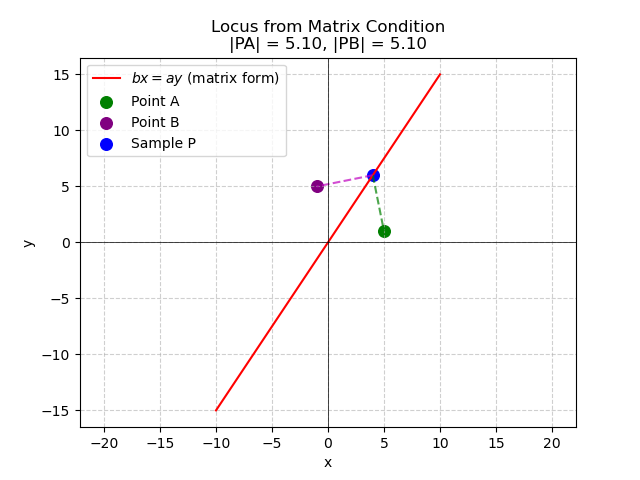
\includegraphics[width=0.9\columnwidth]{figs/Fig1.png}
    \caption{}
    \label{fig:placeholder}
\end{figure}
\end{frame}

\begin{frame}{Direct python code plot}
   
\begin{figure}[H]
    \centering
    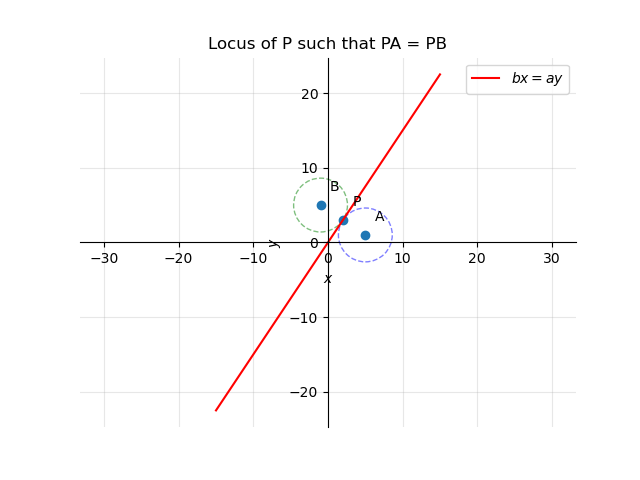
\includegraphics[width=0.9\columnwidth]{figs/fig2.png}
    \caption{}
    \label{fig:placeholder}
\end{figure}

\end{frame}
\begin{frame}[fragile]\frametitle{C Code}
\begin{lstlisting}    

#include <stdio.h>
#include <math.h>

int main() {
    double a, b, x, y;

    // Input parameters
    printf("Enter values of a, b: ");
    scanf("%lf %lf", &a, &b);

    printf("Enter point P(x,y): ");
    scanf("%lf %lf", &x, &y);

    // Define (B - A)
    double BA[2];
    BA[0] = -2 * b;
    BA[1] =  2 * a;
\end{lstlisting}
\end{frame}
\begin{frame}[fragile]\frametitle{C Code}
\begin{lstlisting}   
    // Define P
    double P[2];
    P[0] = x;
    P[1] = y;

    // Compute dot product (B - A)^T P
    double dot = BA[0]*P[0] + BA[1]*P[1];

    printf("Matrix form condition:\n");
    printf("(B - A)^T P = %lf\n", dot);

    if (fabs(dot) < 1e-6)
        printf("=> Point lies on locus (bx = ay)\n");
    else
        printf("=> Point does NOT lie on locus\n");

    return 0;
}
\end{lstlisting}
\end{frame}

\begin{frame}[fragile]\frametitle{Python Code through shared output}
\begin{lstlisting}
import numpy as np
import matplotlib.pyplot as plt

# Parameters
a, b = 2, 3   # You can change values here

# Points
A = np.array([a+b, b-a])
B = np.array([a-b, a+b])
P = np.array([4, 6])   # sample point

# Locus line: bx = ay -> y = (b/a) x (if a != 0)
x_vals = np.linspace(-10, 10, 400)
if a != 0:
    y_vals = (b/a) * x_vals
else:
    x_vals = np.full_like(x_vals, 0)
    y_vals = np.linspace(-10, 10, 400)
\end{lstlisting}
\end{frame}
\begin{frame}[fragile]\frametitle{Python Code through shared output}
\begin{lstlisting}
# Plot locus line
plt.plot(x_vals, y_vals, 'r-', label=r'$bx = ay$ (matrix form)')

# Plot points A, B, and P
plt.scatter(*A, color='green', s=70, label='Point A')
plt.scatter(*B, color='purple', s=70, label='Point B')
plt.scatter(*P, color='blue', s=70, label='Sample P')

# Draw distances PA and PB
plt.plot([P[0], A[0]], [P[1], A[1]], 'g--', alpha=0.7)
plt.plot([P[0], B[0]], [P[1], B[1]], 'm--', alpha=0.7)

# Distance check
dist_PA = np.linalg.norm(P - A)
dist_PB = np.linalg.norm(P - B)

plt.title(f"Locus from Matrix Condition\n|PA| = {dist_PA:.2f}, |PB| = {dist_PB:.2f}")
plt.xlabel("x")
\end{lstlisting}
\end{frame}
\begin{frame}[fragile]\frametitle{Python Code through shared output}
\begin{lstlisting}
plt.ylabel("y")
plt.axhline(0, color='black', columnwidth=0.5)
plt.axvline(0, color='black', columnwidth=0.5)
plt.grid(True, linestyle='--', alpha=0.6)
plt.legend()
plt.axis("equal")
plt.show()
  
\end{lstlisting}
\end{frame}
\begin{frame}[fragile]\frametitle{Direct Python code}
\begin{lstlisting}
import numpy as np
import numpy.linalg as LA
import matplotlib.pyplot as plt

# local imports
from line.funcs import *
from conics.funcs import circ_gen

# Given values
a, b = 2, 3
A = np.array(([a+b, b-a])).reshape(-1,1)   # (5,-3)
B = np.array(([a-b, a+b])).reshape(-1,1)   # (-1,7)
\end{lstlisting}
\end{frame}
\begin{frame}[fragile]\frametitle{Direct Python code}
\begin{lstlisting}
# Choose a point P on line bx = ay
xP = 2
yP = (b*xP)/a
P = np.array(([xP, yP])).reshape(-1,1)

# Distances
dist_PA = LA.norm(P - A)
dist_PB = LA.norm(P - B)

# Generate locus line bx = ay
xx = np.linspace(-15,15,400)
yy = (b*xx)/a

# Plot locus line
plt.plot(xx, yy, 'r', label=r'$bx=ay$ (matrix form)')

# Plot A, B, P
tri_coords = np.block([[A,B,P]])
plt.scatter(tri_coords[0,:], tri_coords[1,:], s=60)
\end{lstlisting}
\end{frame}
\begin{frame}[fragile]\frametitle{Direct Python code}
\begin{lstlisting}

# Labels
vert_labels = ['A','B','P']
for i, txt in enumerate(vert_labels):
    plt.annotate(txt,
                 (tri_coords[0,i], tri_coords[1,i]),
                 textcoords="offset points",
                 xytext=(10,10),
                 ha='center')

# Draw dashed lines PA and PB
plt.plot([A[0,0], P[0,0]], [A[1,0], P[1,0]], 'g--', alpha=0.7)
plt.plot([B[0,0], P[0,0]], [B[1,0], P[1,0]], 'm--', alpha=0.7)

# Circles centered at A and B with radius |PA|
circleA = plt.Circle(A.flatten(), dist_PA, color='blue', fill=False, linestyle='--', alpha=0.4)
circleB = plt.Circle(B.flatten(), dist_PB, color='green', fill=False, linestyle='--', alpha=0.4)
\end{lstlisting}
\end{frame}
\begin{frame}[fragile]\frametitle{Direct Python code}
\begin{lstlisting}

ax = plt.gca()
ax.add_patch(circleA)
ax.add_patch(circleB)

# Axes through origin
ax.spines['top'].set_color('none')
ax.spines['right'].set_color('none')
ax.spines['left'].set_position('zero')
ax.spines['bottom'].set_position('zero')

plt.xlabel('$x$')
plt.ylabel('$y$')
plt.title(f"Locus of P such that PA = PB\n|PA|={dist_PA:.2f}, |PB|={dist_PB:.2f}")
plt.legend()
plt.grid(True, alpha=0.3)
plt.axis('equal')
plt.show()

\end{lstlisting}
\end{frame}

\end{document}